\documentclass[diplom,german]{hgbthesis}
% Zulässige Class Options:
%   Typ der Arbeit: diplom, master, bachelor, praktikum
%               Hauptsprache: german, english
\usepackage{wasysym}
\usepackage{subfig}
\usepackage{todonotes}

\graphicspath{{images/}} % wo liegen die EPS-Bilder?

%\usepackage{natbib}
%\usepackage{url}

\setlength{\parindent}{0ex}
\setlength{\parskip}{1ex}

% Zweifacher Zeilenabstand für Korrekturen
%\renewcommand{\baselinestretch}{2.0}

%%%----------------------------------------------------------
\begin{document}
%%%----------------------------------------------------------
\bibliographystyle{dinat}

%%% Diplomarbeit, Bachelorarbeit, oder Praktikumsbericht?
%%% Entsprechende Bl<F6>cke auskommentieren:

%% Felder für ALLE Arbeiten: --------------------------------
\title{Deep Learning - Lernen von vielschichtigen neuronalen Netzen}
\author{Kjartan Ferstl}
\studiengang{Information Engineering und -Management}
\studienort{Hagenberg}
\abgabemonat{Juni}
\abgabejahr{2014}

%%%----------------------------------------------------------
\frontmatter
\maketitle
\tableofcontents
%%%----------------------------------------------------------

%\chapter{Vorwort} 	% engl. Preface



Dies ist \textbf{Version \hgbthesisDate} der \latex-Dokumentenvorlage für 
verschiedene Abschlussarbeiten an der FH Hagenberg, die mittlerweile auch 
an anderen Hochschulen im In- und Ausland gerne verwendet wird.

Das Dokument entstand ursprünglich auf Anfragen von Studierenden,
nachdem im Studienjahr 2000/01 erstmals ein offizieller
\latex-Grundkurs im Studiengang Medientechnik und -design an der
FH Hagenberg angeboten wurde. Eigentlich war die Idee, die bereits
bestehende \emph{Word}-Vorlage für Diplomarbeiten "`einfach"' in
\latex\ zu übersetzen und dazu eventuell einige spezielle
Ergänzungen einzubauen. Das erwies sich rasch als wenig
zielführend, da \latex, \va was den Umgang mit Literatur und
Graphiken anbelangt, doch eine wesentlich andere Arbeitsweise
verlangt. Das Ergebnis ist -- von Grund auf neu geschrieben und
wesentlich umfangreicher als das vorherige Dokument --
letztendlich eine Anleitung für das Schreiben mit \latex, ergänzt
mit einigen speziellen (mittlerweile entfernten) Hinweisen für \emph{Word}-Benutzer.
Technische Details zur aktuellen Version finden sich in Anhang \ref{ch:TechnischeInfos}.

Während dieses Dokument anfangs ausschließlich für die Erstellung
von Diplomarbeiten gedacht war, sind nunmehr auch  
\emph{Masterarbeiten}, \emph{Bachelor\-arbeiten} und \emph{Praktikumsberichte} 
abgedeckt, wobei die Unterschiede bewusst gering gehalten wurden.

Bei der Zusammenstellung dieser Vorlage wurde versucht, mit der
Basisfunktionalität von \latex das Auslangen zu finden und -- soweit möglich --
auf zusätzliche Pakete zu verzichten. Das ist nur zum Teil gelungen;
tat\-säch\-lich ist eine Reihe von ergänzenden "`Paketen"' notwendig, wobei jedoch
nur auf gängige Erweiterungen zurückgegriffen wurde.
Selbstverständlich gibt es darüber hinaus eine Vielzahl weiterer Pakete,
die für weitere Verbesserungen und Finessen nützlich sein können. Damit kann
sich aber jeder selbst beschäftigen, sobald das notwendige Selbstvertrauen und
genügend Zeit zum Experimentieren vorhanden sind.
Eine Vielzahl von Details und Tricks sind zwar in diesem Dokument nicht explizit
angeführt, können aber im zugehörigen Quelltext jederzeit ausgeforscht
werden.

Zahlreiche KollegInnen haben durch sorgfältiges Korrekturlesen und
konstruktive Verbesserungsvorschläge wertvolle Unterstützung
geliefert. Speziell bedanken möchte ich mich bei Heinz Dobler für
die konsequente Verbesserung meines "`Computer Slangs"', bei
Elisabeth Mitterbauer für das bewährte orthographische Auge und
bei Wolfgang Hochleitner für die Tests unter Mac~OS.

Die Verwendung dieser Vorlage ist jedermann freigestellt und an
keinerlei Erwähnung gebunden. Allerdings -- wer sie als Grundlage
seiner eigenen Arbeit verwenden möchte, sollte nicht einfach
("`ung'schaut"') darauf los werken, sondern zumindest die
wichtigsten Teile des Dokuments \emph{lesen} und nach Möglichkeit
auch beherzigen. Die Erfahrung zeigt, dass dies die Qualität der
Ergebnisse deutlich zu steigern vermag.

Der Quelltext zu diesem Dokument sowie das zugehörige
\latex-Paket sind in der jeweils aktuellen Version online
verfügbar unter
%
\begin{quote}
\url{www.fh-hagenberg.at/staff/burger/diplomarbeit/}
\end{quote}
%
oder auch unter
%
\begin{quote}
\url{http://elearning.fh-hagenberg.at/} \newline
im Kurs "`Anleitung/Vorlage für Master-/Bachelor-/Diplomarbeiten"'.
\end{quote}
%
Trotz großer Mühe enthält dieses Dokument zweifellos Fehler und Unzulänglichkeiten
-- Kommentare, Verbesserungsvorschläge und passende Ergänzungen
sind daher stets willkommen, am einfachsten per E-Mail direkt an mich:
\begin{center}%
\begin{tabular}{l}
\nolinkurl{wilhelm.burger@fh-hagenberg.at} \\
Dr.\ Wilhelm Burger \\
FH Hagenberg -- Digitale Medien\\
Austria
\end{tabular}
\end{center}

\noindent
Übrigens, hier im Vorwort (das bei Diplomarbeiten üblich, bei Bachelorarbeiten 
aber entbehrlich ist) kann man kurz auf die Entstehung  des Dokuments eingehen.
Hier ist auch der Platz für allfällige Danksagungen (\zB an den Betreuer, 
den Begutachter, die Familie, den Hund, ...), Widmungen und philosophische 
Anmerkungen. Das sollte man allerdings auch nicht übertreiben und sich auf 
einen Umfang von maximal zwei Seiten beschränken.




                              %ggfs. weglassen
\chapter{Kurzfassung}

Deep Learning-Algorithmen biete eine Möglichkeit vielschichtige neuronale Netze zu trainieren. Solche Netze kommen in aktuellen Anwendungen zu Erkennung von Objekten in Bildern, Text und Inhalt in Sprache und vielen anderen Gebieten zum Einsatz. Forschungen an den Algorithmen ermöglichen es, die sehr rechenintensiven Algorithmen zu vereinfachen und in großem Stil auf parallelisierten Computersystemen auszuführen. So ist es in einigen Gebieten bereits möglich mit neuronalen Netzen bessere Ergebnisse als mit optimierten mathematischen Verfahren zu erzielen. Im folgenden werden die wesentlichen Algorithmen und Strukturen von neuronalen Netzen aufgearbeitet und die Schwierigkeiten und Lösungsansätze aufgezeigt. Außerdem werden einige aktuelle Anwendungen aus der Bild- und Sprachanalyse betrachtet.
\chapter{Abstract}

\begin{english} %switch to English language rules
Deep learning algorithms enable it to train multi player neural networks. Such networks are used to recognize objects in images, to extract text and content in speach and for many other applications. Research in this area made it possible to reduce the complexity of such algorithms and to compute them in parallel on large scale computer networks. Due to these optimization, it is already possible, to produce better results with an neural network than with existing optimized mathematical algorithms for some applications. This paper is concerned about the major algorithms and structures used for neural networks, the problems they come with and how they can be solved. Moreover some applicactions from object recognition in images and voice analysis are examined.
\end{english}

%%%----------------------------------------------------------
\mainmatter           %Hauptteil (ab hier arab. Seitenzahlen)
%%%----------------------------------------------------------
\chapter{Einleitung}
\label{cha:Einleitung}

Im Zuge einer Projektarbeit wurde ein kleiner autonomer Quadcopter\footnote{Hubschrauber mit vier tragenden Rotoren} für den Innenraum entwickelt. Der Quadcopter verfügt über ein AHRS\footnote{Attitude Heading Reference System}, dieses liefert die Lage im Raum , die Ausrichtung sowie die Beschleunigung. Anhand dieser Daten kann der Quadcopter stabil in der Luft gehalten werden. 

Soll der Roboter einen Punkt im Raum anfliegen, wird die genaue absolute Position des Roboters benötigt. Grundsätzlich könnten die Daten des AHRS dazu verwendet werden. Diese müssten dazu ab Flugbeginn kontinuierlich integriert werden. Dabei werden auch Ungenauigkeiten und Messfehler integriert und der Fehler der neu errechneten Positionen immer größer. Diese Werte können daher nur eine kurze Zeit verwendet werden.

Es wird ein zusätzliches System zum Bestimmen der Position benötigt. Dieses System muss in der Lage sein, eine absolute Position im Innenraum bestimmen zu können und dabei eine ausreichend hohe Auflösung bieten. Solche Systeme werden als LPS\footnote{Local Positioning System} bezeichnet.

Ein LPS liefert, mit einer gewissen Frequenz, eine neue Position. Soll diese erhöht werden, kann die Position mit den Daten des AHRS interpoliert werden. Der dabei auftretende Fehler wird gering gehalten, da nur eine kurze Zeit überbrückt werden muss. 

Das in dieser Arbeit vorgestellte LPS arbeitet mit mehreren Ultraschall-Sendern, welche an möglichst unterschiedlichen Positionen im Raum aufgestellt werden. Anhand von Laufzeitmessungen können Empfänger ihre Position im Raum bestimmen. 

Das verwendete Modulationsverfahren erfordert die zeitgleiche Aussendung der Ultraschallsignale, die Sender müssen daher entsprechend synchronisiert werden. Dazu wird ein sehr schnelles Synchronisationssignal benötigt, welches möglichst zeitgleich bei allen Teilnehmern eintreffen muss.

Um die Signalverarbeitung möglichst einfach zu halten, wurde Ultraschall gewählt. Dieser breitet sich relativ langsam aus und die geringe Frequenz von nur 40 kHz ermöglicht es Empfänger und Sender ohne aufwendige Hochfrequenzbauteile zu implementieren.

Um die Signale aller Sender möglichst zeitgleich aussenden zu können, wird ein Multiplexverfahren benötigt. Da nur eine geringe Bandbreite verfügbar ist, wird dafür CDMA verwendet. Mittels dieser Technik, können die Signale zeitgleich ausgesendet werden und die benötigte Bandbreite wird nur unwesentlich erhöht. \cite{PositionA}, \cite{PositionB}, \cite{BPSK}

Mehr dazu in Kapitel \ref{cha:Multiplex}, \emph{Multiplexverfahren}.



%\section{Gliederung}
%Zu beginn wird im Kapitel "Was ist Ultraschall"\ref{cha:Ultraschall} ein grundlegendes wissen über Ultraschall vermittelt sowie dessen Eigenheiten erläutert.
%Sowie im Kapitel "Ultraschall Erzeugung"\ref{cha:UltraschallErzeugung} Methoden zur Erzeugung von Ultraschall betrachtet. Alternativen zu Ultraschall sind im Kapitel "Alternativen"\ref{cha:Alternativen} zu finden.
%In den Kapiteln "Modulationsverfahren"\ref{cha:Modulationsverfahren} sowie "Multiplexverfahren"  (Kap.~\ref{cha:Multiplexverfahren}) wird näher auf die Möglichkeiten der Datenübertragung sowie dessen Verwendbarkeit im Bezug auf Ultraschallträger eingegangen.
%Für einige Multiplexverfahren werden "Spreitzcodes" benötigt diese werden im gleichnamigen Kapitel(Kap.~\ref{cha:Spreitzcodes}) erläutert, das selbe gilt für das Kapitel "Korrelation"(Kap.~\ref{cha:Korrelation}).
%Im zweiten Teil der Arbeit dreht dich alles um die Positionsberechnung diese wird in den Kapiteln "Abstandsberechnung"(Kap.~\ref{cha:Abstandsberechnung}), 
%"Positionsberechnung 2D"(Kap.~\ref{cha:Positionsberechnung2D}) sowie 
%"Positionsberechnung 3D"(Kap.~\ref{cha:Positionsberechnung3D}) besprochen.
%Im letzten Teil wird die Implementierung beschrieben dies erfolgt in zwei Teile 
%erstens die Hardware Implementation
%"Hardware Sender"(Kap.~\ref{cha:HardwareSender}) sowie
%"Hardware Empfänger	"(Kap.~\ref{cha:HardwareEmpfaenger}),
%zweitens die teilweise Implementierung des VHDL Codes
%"Implementierung BPSK Transmitter"(Kap.~\ref{cha:BPSKTransmitter}) sowie
%"Implementierung BPSK Reciver"(Kap.~\ref{cha:BPSKReciver}).
%Da das Potential der Thematik mit dieser Arbeit noch lange nicht voll ausgeschöpft ist wird im letzten Kapitel "Weitere Arbeit"(Kap.~\ref{cha:WeitereArbeit}) die zukünftige Weiterentwicklung diskutiert.
\chapter{Grundlegendes}
\label{cha:grundlegendes}
% 3 Seiten

\section{Definition}

\section{Entstehung}

\section{Hürden}

\section{Prinzip}

\chapter{Algorithmen}
\label{cha:algorithmen}
% 7 Seiten

%supervised methoden: backpropagation
%unsupervised methoden: restricted boltzmann maschines, autoencoders, sparse coding model


Fokus: viele Daten, parallele Verarbeitung, viel Rechenpower

\section{Backpropagation}

Backpropagation ist ein überwachter Algorithmus zum Trainieren von neuronalen Netzwerken. Bei diesem Algorithmus wird das Netz zunächst mit zufälligen Gewichten belegt. 


training algorithmus für neuronale netzwerke

(sigmoid training function als übertragungsfunktion zwischen neuronenverwendet, e function, einfach zu differenzieren)
-> output = sigmoid(gewicht*input+theta)
theta .. bias

viele inputs in ein neuron


\section{Resctricted Boltzmann Maschines}

\begin{figure}
	\centering
	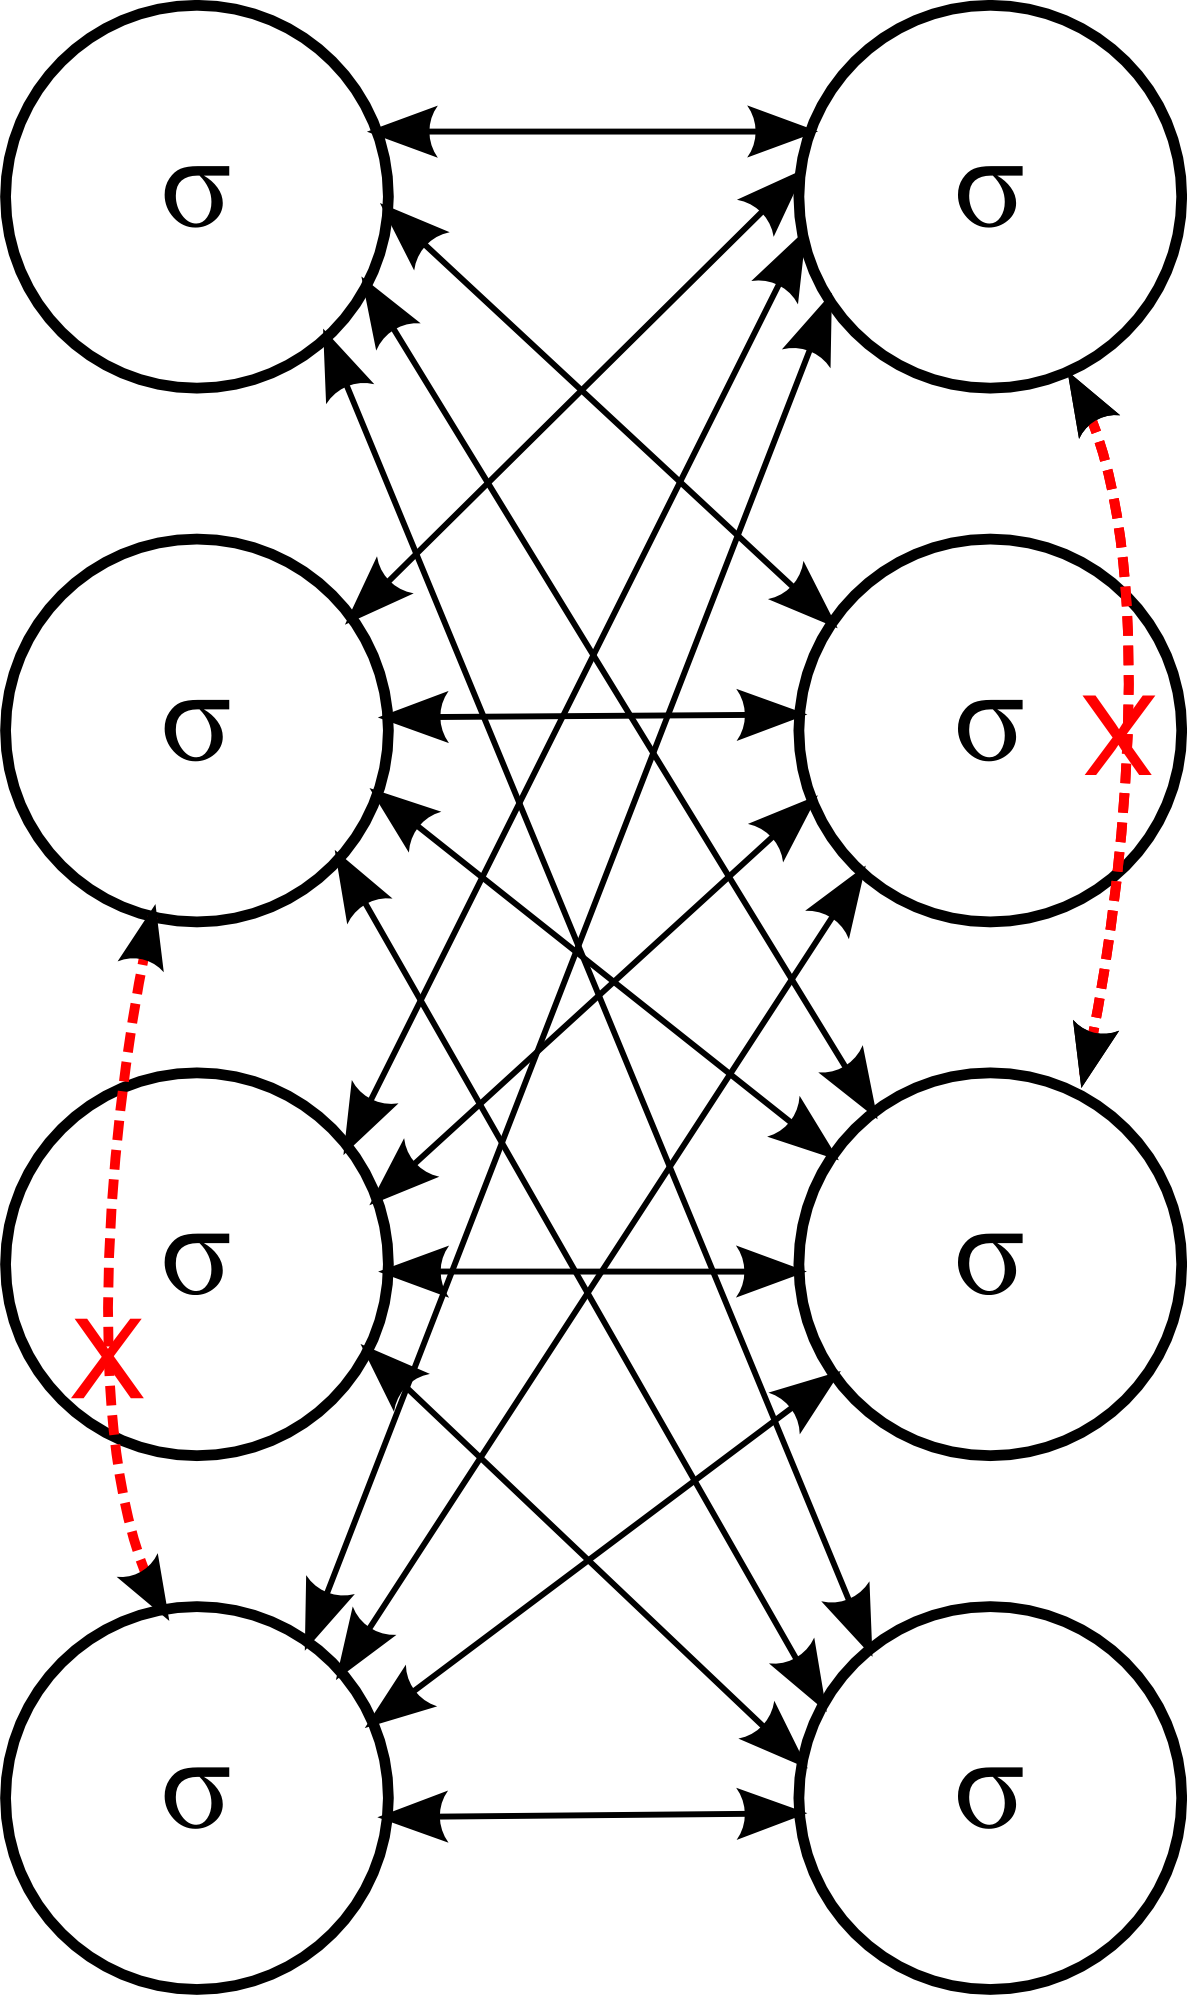
\includegraphics[scale=1]{images/rbm.png}
	\caption{Eine Restricted-Boltzmann-Maschine}
	\label{fig:rbm}
\end{figure}

\begin{figure}%
\centering
\subfloat[Versteckte Schicht berechen]{\begin{minipage}{0.33\textwidth}\centering%
	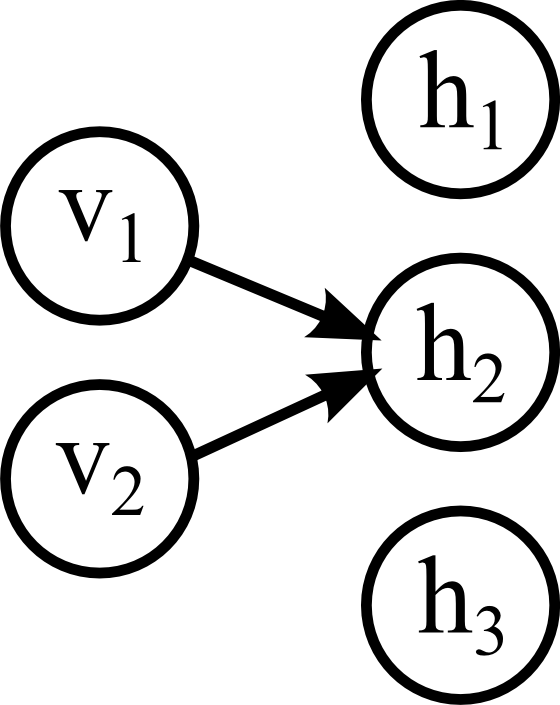
\includegraphics[scale=1]{images/rbm-step1.png}\end{minipage}}
\subfloat[Von der versteckten Schicht zurück rechnen]{\begin{minipage}{0.33\textwidth}\centering%
	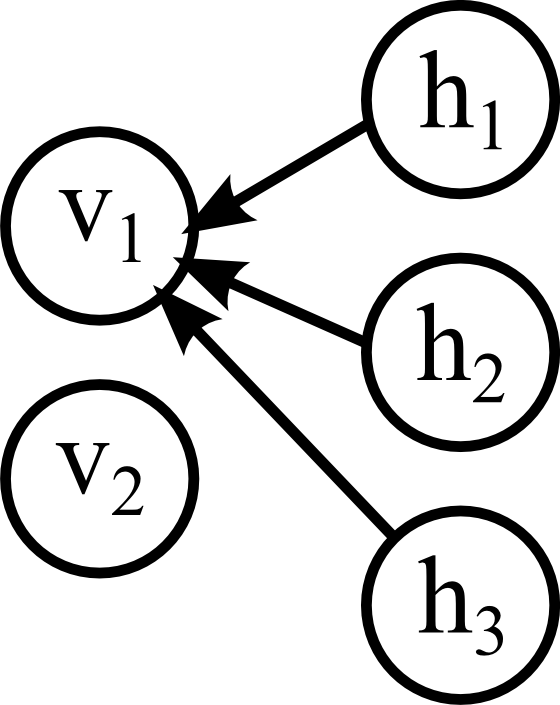
\includegraphics[scale=1]{images/rbm-step2.png}\end{minipage}}
\subfloat[Erneut die versteckte Schicht berechnen]{\begin{minipage}{0.33\textwidth}\centering%
	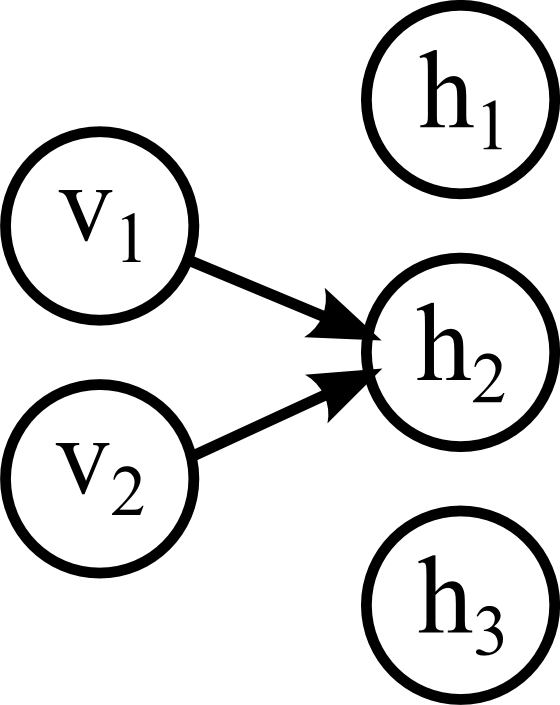
\includegraphics[scale=1]{images/rbm-step3.png}\end{minipage}}
\caption{Die ersten drei Schritte bei der Berechnung von RBMs.}
\label{fig:rbm-steps}
\end{figure}

Uneingeschränkte Neuronale-Netze sind schwierig und aufwendig zu trainieren. Restricted-Boltzmann-Maschines, im weiteren auch als RBMs bezeichnet, sind eingeschränkte neuronale Netzwerke. Wie in Abbildung \ref{fig:rbm} dargestellt, existieren hierbei nur Verbindungen zwischen aneinander liegenden Schichten. Das Modell erlaubt keine Verbindungen von Neuronen zu sich selbst und alle Verbindungen müssen gleichermaßen in beide Richtungen gehen. So lassen sich unter Festlegung der Werte einer Schicht direkt auf die nächste versteckte Schicht weiter gerechnet werden. RBMs arbeiten in der Regel mit bool'schen Werten, lassen sich durch Erweiterung aber auch mit anderen Zahlenräumen verwenden.

RMBs wurden bereits 1986 von Paul Smolensky \todo{ref} unter dem Namen Harmonium erfunden, fanden jedoch erst 1998, rund 10 Jahre später, durch die Entwicklung von effizienten Lernalgorithmen durch Geoffrey Hinton Anwendung.

Zum trainieren von RMBs existieren verschiedene Algorithmen, die meist auf dem Prinzip beruhen, die Gewichte so anzupassen, das das hin und her Rechen zwischen zwei Schichten wieder die Ausgangsdaten ergibt. Im folgenden wird der Algorithmus von Geoffrey Hinton \todo{reference}, der zugleich als der erste effizienten Lernalgorithmus für RMBs gesehen wird, erklärt. 

\subsection{Grundgedanke}

Sind die Werte einer Schicht fixiert, so kann einfach auf die nächste versteckte Schicht weiter gerechnet. Zu beginn werden wird ein Trainingsdatenset an die Eingänge angelegt und die folgenden Operationen wiederholt ausgeführt:

\begin{enumerate}
\item Wahrscheinlichkeit für die versteckten Neuronen berechnen $$p(h_j=1) = \frac{1}{1+e^{-(b_j+\sum_{i}(v_i*w_{ij}))}}$$
\item Werte für die versteckte Schicht aus dem Mittelwert der Wahrscheinlichkeiten berechnen
\item Gradientenmatrix über das dyadische Produkt errechnen $$<v_ih_j> = v*y^T$$
\item Ausgehend von den errechneten versteckten Neuronen, zurück auf die sichtbare Schicht rechnen
\end{enumerate}

Wiederholt man die in der Liste angeführten Schritte sehr oft, so pendeln sich für die Neuronen Werte ein, die im wesentlichen vom Modell und den den Wahrscheinlichkeiten abhängen, jedoch sehr wenig mit den Eingangsdaten zu tun haben. Anhand der Gradientenmatrix des letzten Durchlaufes lässt sich jedoch eine Distanz zum gewünschten Modell herausfinden und so können die Gewichte wie folgt angepasst werden:
$$\Delta\omega_{ij} = \varepsilon (<v_ih_j>^0 -  <v_ih_j>^\infty)$$

Diese Art der Berechnung lieferte sehr gute Modelle. Durch die vielen Iterationen benötigt der Algorithmus sehr viel Rechenzeit und ist daher nicht praxistauglich. Zudem ist es schwierig festzustellen, wie viele Iterationen bis zum Einpendeln notwendig sind.

\subsection{Abkürzung}

Der oben genannte Algorithmus lässt sich in seiner Komplexität erheblich reduzieren, in dem die versteckte Schicht lediglich zwei mal berechnet wird. Geoffrey Hinton hat mit der Vereinfachung gezeigt, dass es möglich ist, bereits mit dem Vergleich der ersten und zweiten Gradientenmatrix möglich ist gute Ergebnisse zu erzielen. Diese Methode wird \emph{Contrastive Divergence} genannt.

Die Regel zur Anpassung der Gewichte lautet dann:
$$\Delta\omega_{ij} = \varepsilon (<v_ih_j>^0 -  <v_ih_j>^1)$$

\subsection{Begründung}

Der Grundgedanke von \emph{Contrastive Divergence} ist, dass das Modell mit Zufallsgewichten weg von den Eingabedaten, hin zu Daten die ihm besser gefallen, wandert. Wenn man erkennt wo hin das Modell die Daten ändert, kann man die Gewichte so adaptieren, dass dem Modell die Eingabedaten am besten gefallen.

Da das Modell nicht genügend Neuronen besitzt um alle Eingabedaten zu speichert, muss es etwas aus den Daten lernen um die Eingänge tatsächlich reproduzieren zu können.



Die Einschränkung vereinfacht das berechnen einer versteckten Schicht und damit das Training des Netzes. Es kann immer eine Schicht als fix angesehen und so zur jeweils zur nächsten weiter gerechnet werden. Initialisiert man das Modell mit Eingangsdaten und zufälligen Gewichten, rechnet immer wieder wiederholt eine Schicht hinein und wieder heraus, während sich die Gewichte nicht ändern, so würde sich das Modell nach sehr langer Zeit auf bestimmte Werte einpendeln bzw. zwischen Werten pendeln. Diese Werte passen gut zu dem Netz, sagen jedoch nicht viel über die Eingangsdaten.

Um das Modell auf die Eingangsdaten zu trainieren, werden diese zunächst als Eingang angelegt und die Gewichte wiederum mit zufälligen Werten initialisiert. Nun wird die zweite und daraus wieder die erste Schicht berechnet. Die Auswirkung auf dein Eingang 
 , und errechnet sich eine wird zu beginn mit zufälligen Gewichten initialisiert, 
 Für das Modell wir eine Energiefunktion aufgestellt, die die Auswirkung Durch die Einschränkung des Netzes kann zur Berechnung der Werte für jeder Übergang von einem Layer auf den nächsten separat betrachtet werden. 
RBMs eignen sich für überwachtes und unüberwachtes Lernen. Beim unüberwachten Lernen, lernt das Netz 
RMBs eignen sich 

type of neural network for unsupervised learning
uses only inputs to train data, no supervised result required
target: extract meaningful features for your data
verfügbarkeit von unlabeled data ausnützen
restriction: allow only connections between the visible and the hidden layers

visible layer, hidden layer
energy function
propability: high energy ergibt low propability
1


\section{Autoencoders}

Autoencoders: Neuronales netz, mit backpropagation trainiert, das zumindest in einer Schicht weniger Neuronen als Eingangsparameter besitzt (bottelneck). Es wir so trainiert, dass der Ausgang dem Eingang entspricht. Steckt man vorne ein Bild hinein und das Netzwerk profezeit am Ausgang das gleiche Bild (mit allen Pixeln), so hat es offensichtlich etwas aus dem Bild gelernt und nicht nur alle Pixel durchgetunnelt (da Anzahl der neuronen kleiner als Anzahl der Pixel).
Es etsteht ein "Hash" für die Bilder - der wieder zurückgewandelt werden kann. Würde man es schaffen, beliebige Eingangsdaten sicher wiederherzustellen, so könnte man davon sprechen, dass das Netz das dahinter liegende System (die Natur) erlernt hat. Im weiteren könnte man so zum Beispiel von Bildern, Videos oder Audiospuren lediglich die Ergebnisse des Netztes speichern und die Eingangsdaten jederzeit widerherstellen. So ließen sich diverse Daten unter umständen erheblich komprimieren.

Füttert man solche Algorithmen mit Bildern und visualisiert die entstandenen Gewichte, so erkennt man, dass solche Algorithmen in erster Instanz meist Kanten und Farbintensitäten in Bildern finden. In der zweiten Schicht findet man einfache Kombinationen dieser Elemente und ab der dritten Schicht werden meist schon sehr brauchbare Neuronen zur vollständigen Objekterkennung ausgebildet.

Blockdiagramm mit mehreren Stufen (siehe Bilderkennung), zum Beispiel Matchen+Normalisieren, Matchen+Normalisieren, . . .


\section{Convolutional Neural Networks}
% als grundlage

\todo{super video, 10 minuten, erkärt das ganze thema: https://www.youtube.com/watch?v=n6hpQwq7Inw}
\todo{bild}
\todo[inline]{bild quelle: http://www.image-net.org/challenges/LSVRC/2012/supervision.pdf}
\todo[inline]{inhalt quelle: wiki, http://googlesystem.blogspot.co.at/2013/06/how-googles-image-recognition-works.html}

erlärung für bilder:
ein neuronales netzwerk, bestehend aus lauter kleineren gruppen an neuronen und vielen schichten. die kleinen Gruppen betrachten Ausschnitte des Bildes und überlappen in ihrer Anordnung. Durch den Blick auf den Ausschnitt eines Bildes wird das dahinter liegende Netzwerk in Teile geteilt und somit die Anzahl der Parameter und somit die Größe und benötigte Trainings und Rechenzeit stark verringert. Durch das Überlappen der einzelnen Bereiche wird berücksichtigt, dass ein späteres High-Level Feature nicht genau in einen Bereich trifft.
Das Überlappen gibt es auch zwischen den einzelnen Layern.
Convolutional networks können auch Layer enthalten, die mehrere Ausgänge von neuronen kombinieren, so genannte polling layer.

Dieser Typ von Netzwerk ist bereits 1980 \todo{paper Kunihiko fukushima}, wurde in den folgenden Jahrzehnten optimiert und erlebte einen Aufschwung durch eine Implementierung auf einer GPU \todo{Dan Ciresan}. Nach weiteren Optimierungen in den vergangen Jahren wurde der Algorithmus unter anderem für ein Projekt von Google \todo{google paper finden} eingesetzt, das nicht zuletzt das so genannte face-neuron ausprägte.

convolution: operation that expresses the amount of overlap with another function
image preprozessing mit gabor filters, erkennt kanten in alle richtungen



\section{betrachtung als restricted bolzman maschine}



\chapter{Anwendungen}
\label{cha:anwendungen}
% 6 Seiten

\section{Bilderkennung}

\section{Spracherkennung}

\section{tech oder elektronik gebiet}
\chapter{Zusammenfassung}
% 2 Seiten

\section{Ergebnisse}

\section{Allgemeines Resümee}

\section{Persönliches Resümee}



%%%----------------------------------------------------------
%%%Anhang
\appendix
%\chapter{Technische Informationen}
\label{ch:TechnischeInfos}

\newcommand*{\checkbox}{{\fboxsep 1pt%
\framebox[1.30\height]{\vphantom{M}\checkmark}}}


\section{Voraussetzungen zum erstellen des VHDL Codes}

Um den VHDL Code synthetisieren zu können wird ein Compiler benötigt.
Wird ein FPGA verwendet so bietet es sich an den Compiler des jeweiligen Herstellers zu verwenden.
Im Fall dieser Arbeit wurde ein Altera FPGA verwendet und dadurch die Entwicklungsumgebung Quartus II von Altera verwendet.
\\\\Altera bietet eine gratis Version von Quartus II an die so genannte Web Version.\footnote{\url{http://www.altera.com/products/software/quartus-ii/web-edition/qts-we-index.html}}
\\\\Um den LogicAnalyser SignalTapII in der Web Version verwenden zu können muss die Talkback Funktion in den Einstellungen aktiviert werden.
\\\\Als Ergänzung zur jeweiligen Entwicklungsumgebung bietet sich Sigasi an ein sehr guter und stabiler VHDL-Editor mit unter Anderem automatischer Vervollständigung und Echtzeit Fehleranzeige.
\\\\Es ist ein kostenlose Universitätsversion von Sigasi verfügbar.\footnote{\url{http://www.sigasi.com/university}}
\\\\Um den VHDL Code zu simulieren wird die Software Questasim oder Modelsim benötigt.
Auch für diese Software ist eine kostenlose Studentenversion verfügbar, nur für Modelsim.\footnote{\url{http://www.mentor.com/company/higher_ed/modelsim-student-edition}}

%\section{Voraussetzungen zum erstellen des Arm-C Codes}
%Dazu werden grundsätzlich 2 Tools benötigt. Einerseits eine Toolchain diese beinhaltet Compiler Linker Debugger usw. sowie eine IDE sprich eine Entwicklungsumgebung.
%\\\\Es gibt eine sehr große Anzahl verschiedener Toolchains am einfachsten zu verwenden sind die YAGARTO Tools. Diese können kostenlos verwendet werden.\footnote{\url{http://www.yagarto.org/}}
%Eine einfache Installation ist ausreichend, es muss nichts weiter beachtet werden.
%\\\\Bezüglich der Entwicklungsumgebung ist es sehr ähnlich es gibt eine Vielzahl meist sehr teurer Tools.
%Eine sehr gute und auch noch kostenlose IDE ist die CoIDE von CooCox.\footnote{\url{http://www.coocox.org/CooCox_CoIDE.htm}}.
%Diese muss lediglich heruntergeladen und installiert werden.

\section{Weitere benötigte Tools}
\begin{itemize}
		\item Matlab\footnote{\url{http://www.mathworks.de/products/matlab/}} mit Simulink sowie dem fdatool zum berechnen der Filter und der Goldsequenzen,
		\item Für die \latex-Version eine funktionierende UTF-8 \latex-Umgebung.
\end{itemize}


     % Technische Erg<E4>nzungen
%\chapter{Inhalt der CD-ROM}
\label{app:cdrom}

\paragraph{Format:} 
		CD-ROM, Single Layer, ISO9660-Format (Standart)%
%\footnote{Verwenden Sie möglichst ein Standardformat, bei DVDs natürlich
%eine entsprechende andere Spezifikation.}

Im Anhang der Bachelorarbeit befindet sich eine CD-ROM welche die Arbeit im PDF-Format sowie im \latex-Format beinhaltet.

Des weiteren befinden sich auf der CD-ROM der erstellte VHDL Code mit allen Aufzeichnungen.

\section{Bachelorarbeit}
Die Bachelorarbeit in digitaler Form.
\begin{FileList}{/Bachelorarbeit}
\fitem{_DaBa.pdf} Diese Diplomarbeit im PDF-Format.
\fitem{latex/} Dieser Ordner beinhaltet die \latex version der Arbeit.%
\end{FileList}

\section{VHDL-Code}
Beinhaltet den VHDL Code für den Sender sowie Empfänger.
\begin{FileList}{/srcVHDL}
\fitem{XXX.vhd} Dies und Das %
\end{FileList}

\section{C-Code}
Erster versuch den Sender in C zu schreiben.
Dabei wurde schnell klar das VHDL der richtige Ansatz ist.
\begin{FileList}{/srcC}
\fitem{XXX.c} Dies und Das %
\end{FileList}

\section{MATLAB}
Dieser Order beinhaltet alle MATLAB Dateien welcher zur Berechnung der Filter sowie zum erstellen der GOLD-Sequenzen erstellt wurden.
\begin{FileList}{/matlab}
\fitem{XXX.m} Dies und Das %
\end{FileList}

\section{HARDWARE}
Schaltpläne für Empfänger / Sender.
\begin{FileList}{/hardware}
\fitem{XXX.sch} Dies und Das %
\end{FileList}

\section{Dokumentation / Referenzen}
Datenblätter der verwendeten Bauteile.
\begin{FileList}{/bauteile}
\fitem{XXX.sch} Dies und Das %
\end{FileList}

Als Referenz verwendete Publikationen.
\begin{FileList}{/papers}
\fitem{XXX.sch} Dies und Das %
\end{FileList}

Aufgezeichnete Daten Oszilloskope, SignalTrapp, Matlab ...
\begin{FileList}{/aufzeichnungen}
\fitem{XXX.sch} Dies und Das %
\end{FileList}

\section{Praktikumsbericht}
\begin{FileList}{/Praktikumsbericht}
\fitem{_PrBericht.pdf} Der Praktikumsbericht im PDF-Format.
\fitem{latex/} Dieser Ordner beinhaltet die \latex version des Berichtes.%
\end{FileList}     % Quelltext dieses Dokuments
%\chapter{Chronologische Liste der Änderungen}


\begin{sloppypar}
\begin{description}
%
\item[2013/25/08]
Initial Version!
%

\end{description}

\end{sloppypar}




%\section*{To Do} 
%\begin{itemize}
%\item Inkscape
%\item biblatex Bib-Driver für audio, video etc. ergänzen.
%\item Mathematik umbauen, typische Fehler stärker berücksichtigen (ua. Leerzeilen vor/nach Gleichungen).
%\item Literaturempfehlungen zum Schreiben von Diplomarbeiten
%\item Hinweise für Literatursuche (Bibliotheksverbund, CiteSeer,...)
%\end{itemize}





     % Chronologische Liste der <C4>nderungen

%%%----------------------------------------------------------
\clearpage
\addcontentsline{toc}{chapter}{\bibname}
%\bibliographystyle{alphaurlde}
%\bibliographystyle{gerabbrv}
%options: babplain, babunsrt, bababbrv, babalpha, babamspl,
%         babplain-fl etc: first/lastname
%         babplain-lf etc: last/firstname
\bibliography{bibliography}     %BibTeX-Datei literatur.bib


%%%----------------------------------------------------------

%%%Messbox zur Druckkontrolle
\chapter*{Messbox zur Druckkontrolle}



\begin{center}
{\Large --- Druckgröße kontrollieren! ---}

\bigskip

\Messbox{100}{50} % Angabe der Breite/Hoehe in mm

\bigskip

{\Large --- Diese Seite nach dem Druck entfernen! ---}

\end{center}



\end{document}